\scnheader{Введение в язык графического представления баз знаний ostis-систем}
\scnidtf{Введение в SCg-код}
\scnreltovector{конкатенация сегментов}{Первый сегмент Введения в SCg-код;Описание Ядра SCg-кода;Описание Первого расширения Ядра SCg-кода;Описание Второго расширения Ядра SCg-кода;Описание Третьего расширения Ядра SCg-кода;Описание Четвертого расширения Ядра SCg-кода;Описание Пятого расширения Ядра SCg-кода;Описание Шестого расширения Ядра SCg-кода;Описание Седьмого расширения Ядра SCg-кода;Последний сегмент Введения в SCg-код}

\scnheader{следует отличать*}
\scnhaselement{\scnset{\textit{SCg-код}; \textit{Введение в SCg-код}}}
\scnhaselement{\scnset{\textit{Ядро SCg-кода}; \textit{Описание Ядра SCg-кода}}}
\scnhaselement{\scnset{\textit{Первое расширение Ядра SCg-кода}; \textit{Описание Первого расширения Ядра SCg-кода}}}

\scnsourcecomment{То есть следует отличать саму описываемую сущность и текст, являющийся описанием этой сущности}

\scnheader{SCg-код}
\scnidtf{Semantic Code graphical}
\scnidtf{Язык визуального (графического) представления баз знаний ostis-систем}
\scnexplanation{SCg-код представляет собой способ визуализации sc-текстов (sc-конструкций) в виде рисунков этих конструкций. Подчеркнем, что абстрактная графовая структура и её рисунок (графическое изображение) -- это не одно и тоже даже, они изоморфны друг другу. SCg-код рассматривается нами как \textit{объединение*} нескольких его подъязыков, в число которых входит Ядро SCg-кода, обеспечивающее изоморфное графическое изображение любого sc-текста, а также несколько направлений расширения этого ядра, обеспечивающих повышение компактности и и читабельности текстов SCg-кода (sc.g-текстов, sc.g-конструкций).}

\scnendstruct

\scnsegmentheader{Описание Ядра SCg-кода}

\scnstartsubstruct

\bigskip
\scnfilelong{Алфавиту SC-кода взаимно однозначно соответствует алфавит \textit{Ядра SCg-кода} (алфавит sc.g-элементов, графически изображающих sc-элементы). Все sc-узлы, не являющиеся знаками файлов в тексте (конструкции) \textit{Ядра SCg-кода} изображаются в виде небольших чёрных кругов одинакового радиуса, который обозначим через $r$, и точная величина которого зависит от масштаба отображения sc.g-конструкции. Каждое \uline{sc-ребро} в \textit{Ядре SCg-кода} изображается в виде линии произвольной формы не имеющий самопересечений и имеющей толщину, равную примерно $r/8$.

Каждая \uline{sc-дуга} в \textit{Ядре SCg-кода} изображается в виде линии произвольной формы, не имеющей самопересечений, имеющей толщину равную $r/8$ и имеющей изображение стрелочки на одном из концов этой линии. 

Каждая входящая в sc-конструкцию \uline{базовая sc-дуга} в \textit{Ядре SCg-кода} изображается в виде линии произвольной формы, не имеющий самопересечений, имеющий толщину $r/4$, и имеющей изображение стрелочки на одном из ее концов. 

Каждый входящий в sc-конструкцию \uline{sc-узел}, имеющий содержимое, в \textit{Ядре SCg-кода} изображается в виде прямоугольника произвольного размера с толщиной линии $r/6$. Внутри этого прямоугольника отображается файл, обозначаемый изображаемым sc-узлом. Если нет необходимости изображать в тексте сам файл, обозначаемый sc-узлом, имеющим содержимое, то такой sc-узел в Sc.g-тексте изображается в виде прямоугольника со сторонами $2r$ по вертикали и $4r$ по горизонтали.

Представим таблицу соответствия между \textit{Алфавитом SC-кода} (Алфавитом абстрактных элементов sc-конструкций) и \textit{Алфавитом Ядра SCg-кода} (Алфавитом графических примитивов, составляющих конструкции Ядра SCg-кода и являющихся изображениями sc-элементов).}

\scnheader{Таблица. Алфавит Ядра SCg-кода}
\scneqfile{\\
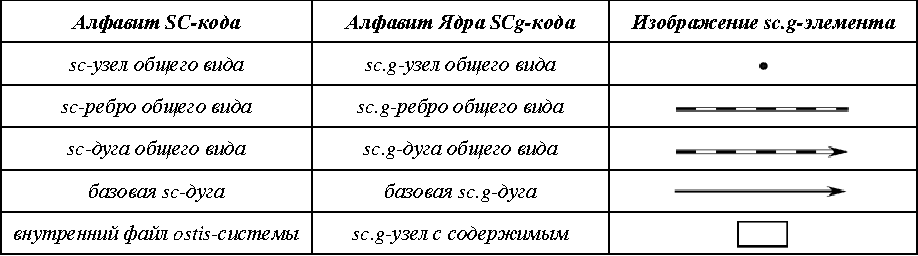
\includegraphics{figures/intro/SCg-core-alphabet.pdf}\\
}

\scnheader{Описание Ядра SCg-кода}
\scnseminclusion{Трудно сразу поверить, что на основе такого простого алфавита можно построить удобный и \uline{универсальный} графовый язык. В рамках \textit{Описания Технологии OSTIS} мы постараемся Вас в этом убедить. Кроме того, нас не должна настораживать простота алфавита, поскольку человечество имеет большой опыт кодирования, хранения в памяти и передачи по каналам связи самых различных информационных ресурсов, используя алфавит, состоящий только из двух классов элементов -- единиц и нулей. 

Мы ведем речь о принципиально ином (графовом) способе кодирования информации в компьютерных системах, но стараемся при этом свести это кодирование к достаточно простому алфавиту хотя бы для того, чтобы искусственно не усложнять проблему создания нового поколения компьютеров, основанных на указанном способе кодирования информации. 

Расширения \textit{Ядра SCg-кода} рассмотрим как направления перехода от текстов \textit{Ядра SCg-кода} к более компактным текстам. Но, поскольку это приводит к усложнению \textit{Синтаксиса SCg-кода} и, в первую очередь, к расширению \textit{Алфавита SCg-кода}, делать такие расширения необходимо обоснованно с учетом частоты встречаемости в рамках \textit{баз знаний ostis-систем} соответствующих фрагментов.}

\scnendstruct


\scnsegmentheader{Описание Шестого расширения Ядра SCg-кода}

\scnstartsubstruct

\bigskip
\scnfilelong{\textbf{\textit{Шестое расширение Ядра SCg-кода}} -- это введение в SCg-код sc.g-контуров, sc.g-рамок и sc.g-шин как средств структуризации sc.g-текстов и повышения наглядности при их размещении. Подчеркнем, что и sc.g-контуры, и sc.g-шины, и sc.g-рамки являются специальными видами sc.g-элементов. При этом sc.g-контуры и sc.g-рамки являются sc.g-ограничителями (ограничителями SCg-кода).

Каждый sc.g-контур изображается (в 2D-модификации) в виде замкнутой ломаной линии, ограничивающей некоторый фрагмент sc.g-текста и обозначает множество всех \uline{sc-элементов}, sc.g-изображения которых оказались внутри этого контура.

Обозначение множества sc-элементов, изображаемое sc.g-контуром, может быть как константным, так и переменным. Соответственно этому линия, изображающая sc.g-контур может быть: 

\begin{scnitemize}
\item неточечной линией без пропусков,
\item точечной линией без пропусков,
\item неточечной пунктирной линией,
\item точечной пунктирной линией.
\end{scnitemize}

Семантическим эквивалентом sc.g-контуру является sc.g-узел, обозначающий sc-структуру. Использование sc.g-контура вместо указанного sc.g-узла исключает необходимость явно изображать SC-дуги принадлежности, выходящие из этого sc.g-узла. Это существенно повышает уровень наглядности sc.g-текста.

Если представленный внутри sc.g-контура текст не является sc.g-текстом, то считается, что что на самом деле внутренностью sc.g-контура является sc.g-текст, являющийся результатом переводя предоставленного текста в SCg-код.

Каждая sc.g-рамка является ограничителем изображения файла, обозначаемого этой sc.g-рамкой. Таким образом, sc.g-рамка может быть sc.g-ограничителем не только sc.g-текстов, но и любых других инородных для SCg-кода информационных конструкций, изображаемых на плоскости.

Семантическим эквивалентом sc.g-рамок являются sc.g-узлы следующего вида (\textit{Файл. Примеры SCg-рамок различного вида}).

Соответственно этому, sc.g-рамки всегда являются константными, хотя переменные, значениями которых являются sc.g-узлы, обозначающие файлы-ostis-систем, существуют, но  содержимого эти переменные иметь не могут.

Каждая sc.g-шина представляет собой замкнутую или незамкнутую линию, которая инцидентна только одному sc.g-элементу и семантически ему эквивалентна. Идея введения sc.g-шин заключается в увеличении «размеров» sc.g-элементов для расширения их области инцидентности. Особенно актуально это для sc.g-узлов, имеющих большое число инцидентных им sc.g-коннекторов.}

\scnheader{Файл. Примеры SCg-рамок различного вида}
\scneq{\scnfileshort{c.70}}

\scnendstruct

\scnsegmentheader{Описание Седьмого расширения Ядра SCg-кода}

\scnstartsubstruct

\bigskip
\scnfilelong{\textbf{\textit{Седьмое расширение Ядра SCg-кода}} -- это переход от 2D-изображений sc.g-текстов к 3D-изображениям.
Одним из вариантов трехмерного изображения sc.g-текстов является следующий:

\begin{scnitemize}
\item все sc.g-узлы изображаются, как и ранее, \uline{плоскими} графическими примитивами. При изменении точки просмотра они \uline{всегда} "поворачиваются"\ параллельно плоскости экрана, но их масштаб (размер на экране) при удалении от  точки просмотра \uline{уменьшается};
\item аналогичным "плоским"\ образом изображаются sc.g-рамки с их "внутренним"\ содержанием, а также внешние идентификаторы, приписываемые sc.g-элементам;
\item sc.g-коннекторы изображаются \uline{непересекающимися} линиями в трехмерном пространстве (заметим, что при изображении sc.g-текстов на плоскости пересечение sc.g-коннекторов часто снижает наглядность, "читательность"\ sc.g-текстов). Т.е. sc.g-коннекторы, которые на плоскости изображаются двойными линиями, в пространстве  цилиндрическими, "трубчатыми линиями"\ с находящейся внутри тонкой, но просвечивающейся осевой линией;
\item sc.g-контур в пространстве визуализируется несколькими (!) специального вида точками -- например там, где есть точки инцидентности sc.g-контура с \uline{внешними} sc.g-коннекторами. При этом sc.g-контур становится виден только по команде просмотра указываемого контура (указание контура – это указание одной из его точек инцидентности). По этой команде цветом выделяются все граничные точки контура (точки инцидентности) и все внутренние sc.g-элементы контура. Если просматривается  несколько контуров, то используется несколько цветов.
\end{scnitemize}

Вторым вариантом 3D-визуализации sc.g-текстов является размещение sc.g-текстов на параллельных плоскостях (слоях) с “прошивками”\ между этими слоями, соединяющими синонимичные sc.g-узлы, т.е. sc.g-узлы, имеющие одинаковые приписываемые им внешние идентификаторы. Такой вариант плоской, но многослойной визуализации sc.g-текстов дает возможность широко использовать те средства просмотра и редактирования sc.g-текстов, которые разработаны для плоской их визуализации.}

\scnendstruct